\documentclass[11pt,a4paper]{article}
\usepackage[utf8]{inputenc}
\usepackage[T1]{fontenc}
\usepackage[margin=2.5cm]{geometry}
\usepackage{amsmath,amssymb}
\usepackage{booktabs,array}
\usepackage{xcolor}
\usepackage{tcolorbox}
\tcbuselibrary{skins,breakable}
\usepackage{tikz}
\usetikzlibrary{arrows.meta,positioning,shapes.geometric,calc,fit,backgrounds}
\usepackage{hyperref}
\hypersetup{colorlinks=true,linkcolor=blue!60!black,urlcolor=blue!60!black,
            citecolor=blue!60!black}
\setlength{\emergencystretch}{2em}
\usepackage{enumitem}
\usepackage[numbers,sort&compress]{natbib}

\definecolor{boxblue}{RGB}{220,235,255}
\definecolor{boxorange}{RGB}{255,240,210}
\definecolor{boxgreen}{RGB}{220,245,220}

\newcommand{\term}[1]{\textbf{#1}}
\newcommand{\lean}[1]{%
  \penalty-100
  \begingroup\def\_{\textunderscore\allowbreak}\texttt{#1}\endgroup}
\newcommand{\CatAL}{\ensuremath{\mathbf{A}_{\rm Lean}}}
\newcommand{\CatAD}{\textbf{A/D}}
\newcommand{\CatA}{\textbf{A}}

\newcommand{\TutorialDOI}{10.5281/zenodo.20669162}
\date{2026}

\title{\textbf{The Problem of Physics:}\\[6pt]
\large Why the Standard Model Needs an Explanation\\[8pt]
\normalsize
\href{https://novaspivack.com/research}{novaspivack.com/research}\quad
\href{https://doi.org/10.5281/zenodo.20560550}{P48 complete theory monograph}\\[4pt]
\small\href{https://doi.org/\TutorialDOI}{doi.org/\TutorialDOI}
  \textit{(registration pending)}\\[4pt]
\normalsize\textit{UGP Physics Tutorial Series}}
\author{Nova Spivack}

\begin{document}
\setcounter{tocdepth}{2}
\maketitle
\tableofcontents
\newpage

\begin{tcolorbox}[colback=blue!6,colframe=blue!40!black,
  title=\textbf{UGP Physics Tutorial Series}]
\textbf{Prerequisites (read first):} None --- this is a foundational tutorial.\\[4pt]
\textbf{Next tutorials:}
  \href{https://doi.org/10.5281/zenodo.20657889}{\emph{The GTE Polynomial: A Step-by-Step Cheat Sheet}}
  $\cdot$
  \href{https://doi.org/10.5281/zenodo.20657895}{\emph{Perfect Self-Containment and MDL}}\\[4pt]
\textbf{See also:}
  \href{https://doi.org/10.5281/zenodo.20657872}{\emph{The Levels of the Theory}}
  $\cdot$
  \textbf{P48} (synthesis monograph,
  \href{https://doi.org/10.5281/zenodo.20560550}{doi.org/10.5281/zenodo.20560550})
\end{tcolorbox}

\begin{tcolorbox}[colback=boxgreen,colframe=green!50!black,
  title=\textbf{Claim-Strength Taxonomy}]
Throughout this tutorial, results are labeled with a confidence grade:
\begin{itemize}[itemsep=2pt]
  \item \textbf{$\mathbf{A}_{\rm Lean}$ (CatAL)} --- Machine-certified in Lean~4 with zero \texttt{sorry} and zero custom axioms.  Independently verifiable by anyone with Lean installed.
  \item \textbf{A/D (CatAD)} --- Analytically derived with full derivation, computationally confirmed.  Not yet machine-certified.
  \item \textbf{A (CatA)} --- Analytically derived; derivation complete but not independently machine-certified.
  \item \textbf{A/D (conditional)} --- Derived under a named, stated premise; the premise is itself an open problem or a CatB assumption.
  \item \textbf{B (CatB)} --- A stated working hypothesis or structural premise; not yet derived.
\end{itemize}
\end{tcolorbox}

%─────────────────────────────────────────────────────────────────────────────
\section{The Most Successful Theory in the History of Science}
\label{sec:success}
%─────────────────────────────────────────────────────────────────────────────

\begin{tcolorbox}[colback=boxblue,colframe=blue!40!black,
  title=The central paradox]
The Standard Model of particle physics is the most precisely tested theory
in the history of science --- and simultaneously the theory with the most
embarrassing structural gap.
It works with extraordinary accuracy.
It also cannot explain itself.
\end{tcolorbox}

The \term{Standard Model} (SM) is the physical theory describing all known
elementary particles and three of the four fundamental forces (electromagnetic,
weak nuclear, and strong nuclear).
It predicts the anomalous magnetic moment of the electron to twelve significant
figures~\cite{SpivackGTECompleteFramework}.
It predicted the existence of the $W$ and $Z$ bosons before they were discovered
in 1983.
It correctly describes the quark structure of the proton and neutron.
Every experimental result ever obtained has been consistent with SM predictions.

That record of success is not in question.
The problem is structural: \textbf{the Standard Model does not derive its own constants.}

\subsection{The free parameters}

To make its predictions, the SM requires a set of numerical inputs to be
measured by experiment and inserted by hand.
These are called \term{free parameters} --- ``free'' because the theory
places no restriction on what value they could take.
Change any of them and the SM remains a logically consistent theory;
it just describes a different universe with different particles and forces.

In the strictest count, the SM has 19 free parameters.
Adding the three neutrino masses and the neutrino mixing angles brings the
tally to 25.
Including the cosmological constant and related cosmological quantities,
the extended census reaches 26--28.

\begin{tcolorbox}[colback=boxorange,colframe=orange!60!black,
  title={The 25 standard model free parameters},breakable]
\begin{itemize}[itemsep=2pt]
  \item \textbf{Gauge couplings (3):} the strengths of the strong force
        ($\alpha_s$), the weak force, and electromagnetism ($\alpha$).
  \item \textbf{Higgs sector (2):} the Higgs vacuum expectation value $v$
        and the Higgs mass $m_H$.
  \item \textbf{Quark masses (6):} up, down, strange, charm, bottom, top.
  \item \textbf{Charged lepton masses (3):} electron, muon, tau.
  \item \textbf{Quark mixing (4):} three mixing angles and one CP-violating phase
        (the CKM matrix).
  \item \textbf{Neutrino mixing ($\geq 4$):} three mixing angles and at least
        one CP-violating phase (the PMNS matrix).
  \item \textbf{Strong CP angle:} $\theta_{\rm QCD}$, which controls CP violation
        in the strong force.
  \item \textbf{Cosmological parameters:} the cosmological constant $\Lambda$,
        dark matter density, and related quantities.
\end{itemize}
None of these 25--28 numbers is predicted by the Standard Model.
Each is measured and inserted.
\end{tcolorbox}

\subsection{Why free parameters are not explanations}

A free parameter is a measurement --- the outcome of an experiment.
It is not a derivation.

When you measure the electron mass $m_e = 0.511$~MeV and put it into
the Standard Model, the SM correctly predicts everything that depends
on $m_e$: the size of atoms, the chemistry of life, the behavior of
electric currents.
That predictive success is real and valuable.

But the question ``why does the electron have that particular mass and not
some other?'' is unanswered.
The SM cannot ask it.
The SM treats the electron mass as an input, like a knob set by experiment.

A complete theory of physics would answer the question.
It would say: the electron mass has that value \emph{because} of this
deeper structure, and we could have derived the value without measuring it.
The Standard Model is not that theory.

%─────────────────────────────────────────────────────────────────────────────
\section{Four Deep Problems Inside the Standard Model}
\label{sec:deep}
%─────────────────────────────────────────────────────────────────────────────

Among the 25 free parameters, four sub-problems stand out as particularly
deep --- not just numerical gaps but structural failures that indicate
something fundamental is missing.

\subsection{The hierarchy problem}

Gravity is approximately $10^{32}$ times weaker than the weak nuclear force.
Newton's constant $G_N$ appears in the SM as a dimensionful input with
no derivable value.
But the deeper puzzle concerns the Higgs boson.

The Higgs mass is approximately 125~GeV.
Quantum mechanics predicts that quantum corrections --- the effects of
short-distance physics --- should drag the Higgs mass up to the
\term{Planck scale} ($\approx 10^{19}$~GeV), which is $10^{17}$ times larger
than the observed value.
To get the observed Higgs mass in the SM, you must either accept that
two enormous numbers cancel to 17 decimal places by coincidence
(extreme fine-tuning), or invoke new physics that cancels the corrections.

This is the \term{hierarchy problem}: the gap between the electroweak scale
($\sim 100$~GeV) and the Planck scale ($\sim 10^{19}$~GeV) appears unnatural
in the Standard Model.
The Generative Triple Evolution (GTE) framework, described in the companion
tutorials, resolves this gap structurally: the electroweak scale is set by a
fixed-point equation with no fine-tuning~\cite{SpivackSRRG}.

\subsection{The strong CP problem}

The SM Lagrangian (the equation that encodes all SM physics) admits a term
that would cause the strong nuclear force to violate \term{CP symmetry}
--- the symmetry between matter and antimatter.
The coefficient of that term is $\theta_{\rm QCD}$.
There is no argument in the SM for why $\theta_{\rm QCD}$ should vanish;
it could take any value between 0 and $2\pi$.

Experiment constrains $|\theta_{\rm QCD}| < 10^{-10}$ --- essentially zero
to ten decimal places.
Why is a parameter that could be anything so extraordinarily close to zero?
This is the \term{strong CP problem}.

The standard proposed resolution invokes the \term{Peccei--Quinn axion}:
a hypothetical new particle whose dynamics relax $\theta_{\rm QCD}$ to zero.
Decades of dedicated searches have found no axion.
In the GTE framework, $\theta_{\rm QCD} = 0$ exactly follows from the symmetry
group of the theory, with three independent machine-certified proofs
and no axion required or predicted~\cite{SpivackGTECompleteFramework}.

\subsection{The three-generation puzzle}

Why are there exactly three families of quarks and leptons?
The SM predicts nothing about the number of generations.
There happen to be three: (electron, muon, tau), (up/down, charm/strange, top/bottom).
Anomaly cancellation in the SM requires quarks and leptons to come in equal
numbers of generations, but imposes no constraint on what that number is.
One generation, four generations, and seventeen generations are all perfectly
consistent SM theories --- just not the universe we live in.

In the GTE framework, $N_{\rm gen} = 3$ is forced by independent structural constraints,
including machine-certified mechanisms
(\lean{psc\_enumeration\_forces\_ngen\_3}, \CatAL;
\lean{fmdl\_gen1\_is\_garden\_of\_eden}, \CatAL).
Seven independent structural constraints are simultaneously certified in a single bundle
\mbox{(\lean{ngen\_universality\_seven\_constraints}, \CatAL)}, with an eighth
constraint conditional on the carrier-pricing identification completing the assembly
\mbox{(\lean{ngen\_universality\_master}, \CatAL)}~\cite{SpivackGTECompleteFramework}.

\subsection{The measurement problem}

Quantum mechanics predicts the \emph{probability} of each experimental outcome
via the \term{Born rule}: $P(k) = |\langle k | \psi \rangle|^2$.
This rule was introduced as an assumption (a postulate) in 1926 by Max Born.
It has never been derived from more fundamental principles.

Why does a quantum system in a definite mathematical state produce only
probabilistic measurement outcomes?
What causes the ``collapse'' from a superposition of possibilities to a
single result?
This is the \term{measurement problem}, and it has resisted resolution for
a century.
In the GTE framework, the Born rule is derived from four independent routes,
two of which are machine-certified in Lean~4 at \CatAL\ with zero custom
axioms (\lean{born\_rule\_unconditional})~\cite{SpivackBornRule}.

%─────────────────────────────────────────────────────────────────────────────
\section{What Would ``Explaining'' Physics Actually Mean?}
\label{sec:explain}
%─────────────────────────────────────────────────────────────────────────────

\begin{tcolorbox}[colback=boxgreen,colframe=green!50!black,
  title=The distinction that matters]
A \textbf{measurement} tells you the value of a parameter.
A \textbf{derivation} shows you why that value is what it is ---
before you measure it.
The Standard Model can measure; it cannot derive.
A complete theory of physics would derive.
\end{tcolorbox}

To make the distinction concrete, consider Newton's constant $G_N$.
The SM treats $G_N$ as a free input.
The GTE framework derives it from the orbit combinatorics of a finite group
($F_{21} = \mathbb{Z}_7 \rtimes \mathbb{Z}_3$), with a result
$M_{\rm Pl}/m_\tau = F_{21}^{10} \times |\mathbb{Z}_7|^{7/2}$
that agrees with the measured value to $0.040\%$~\cite{SpivackGTECompleteFramework}.
No gravitational input enters the derivation.

\subsection{The three requirements for a genuine derivation}

A genuine explanation of the SM parameters must meet three criteria:

\begin{enumerate}[itemsep=4pt]
  \item \textbf{Zero free parameters.}
        No SM constant may be used as an input on the way to deriving another.
        Every constant is an output.
        If any constants are fitted to data during the derivation, the derivation
        is circular.

  \item \textbf{Prior to measurement.}
        The derivation must not use the measured value as an implicit guide.
        In practice, this means a machine-certified proof --- a formal proof
        system that has no knowledge of what the Standard Model predicts
        and cannot unconsciously steer the algebra toward the known answer.

  \item \textbf{Falsifiable.}
        A genuine derivation makes a specific numerical prediction.
        If the prediction disagrees with measurement, the theory is wrong.
        A framework that can accommodate any experimental outcome by adjusting
        assumptions is not a derivation; it is a description.
\end{enumerate}

The GTE framework satisfies all three requirements.
Every foundational result is proved in Lean~4 with zero sorry (no gaps) and
zero custom axioms beyond Lean's standard foundations.
The key uniqueness result
(\lean{mdl\_total\_z7z3\_strictly\_beats\_z5z3}, \CatAL)
was verified by a machine that does not know what the Standard Model
predicts~\cite{SpivackGTECompleteFramework}.

\subsection{The difference between a prediction and a measurement}

It is worth dwelling on what it means to predict rather than fit.

The SM has 25 free parameters.
If you are allowed to adjust 25 knobs after seeing the experimental data,
you can fit almost anything.
A theory with 25 free parameters that fits 25 observations is not impressive;
it is tautological.
The SM's extraordinary success comes from a smaller number of parameters
fitting a much larger number of predictions --- but the parameters are
still fitted, not derived.

A theory with \emph{zero} free parameters that correctly predicts 40
independent observables without fitting any of them is a different kind
of achievement.
The probability that a zero-free-parameter theory matches 40 independent
predictions all within $1\sigma$ by coincidence is approximately
$(0.683)^{40} \approx 5 \times 10^{-7}$.
This is the GTE result as of the synthesis monograph P48~\cite{SpivackGTECompleteFramework}.

%─────────────────────────────────────────────────────────────────────────────
\section{Three Classes of Attempted Solutions}
\label{sec:solutions}
%─────────────────────────────────────────────────────────────────────────────

The SM's parameter problem has been recognized since the 1970s.
Three broad classes of attempted solutions have been proposed.

\subsection{Fine-tuning and anthropic reasoning}

One response is to deny that the problem needs an explanation.
The SM parameters are what they are; they happen to be compatible with the
existence of observers like us; that is why we observe these values and not others.

This \term{anthropic reasoning} sounds plausible, but it is not science.
It converts the question ``why does the electron have this mass?'' into
``only if it had this mass could we be here to ask'' --- which is true but
uninformative.
Anthropic reasoning cannot predict anything.
It can be used to ``explain'' any set of constants, which means it explains none of them.

\subsection{Landscape and multiverse approaches}

String theory and related frameworks produce a \term{landscape}: an enormous
space of possible physical laws, with approximately $10^{500}$ distinct
``vacuum states,'' each corresponding to a different set of SM parameters.
Our universe is argued to be one point in this landscape, with the observed
constants determined by which vacuum we happen to inhabit.

The landscape approach promotes anthropic reasoning to a formal framework.
It has a genuine mathematical consistency: string theory is a rich and
self-consistent mathematical system.
The problem is scientific: a theory that can produce $10^{500}$ distinct
sets of physical constants can accommodate any observation.
A theory that can explain anything explains nothing.
The landscape is not falsifiable.

\subsection{Structural derivation}

The third approach --- the one taken by the GTE framework --- holds that
the SM parameters are not free at all.
They are \emph{theorems}: consequences of a deeper mathematical structure
that selects exactly one set of physical laws, with no adjustable inputs.

The selection principle in GTE is \term{Perfect Self-Containment} (PSC):
the universe must be its own complete description.
A universe that required an external description would have an ``outside,''
which contradicts the definition of a universe.
PSC, combined with Presentation Invariance (the requirement that the
description be independent of how it is presented), is provably equivalent
to \term{Minimum Description Length} (MDL): the universe must be
the shortest possible self-consistent description~\cite{SpivackGTECompleteFramework}.

This is not metaphysics.
It is a mathematical theorem with a machine-certified proof.
The MDL principle selects a unique structure
($\mathbb{Z}_7 \times \mathbb{Z}_3$, implemented as the
19-bit polynomial $p(L,C,R) = C + R - CR - LCR \pmod{7}$),
and the SM parameters are then derived from that structure.

%─────────────────────────────────────────────────────────────────────────────
\section{A Century of Unification: What Has Been Achieved and What Remains}
\label{sec:history}
%─────────────────────────────────────────────────────────────────────────────

To place the GTE approach in context, it helps to review what physics has
already unified and what structural gap remains.

\begin{figure}[h]
\centering
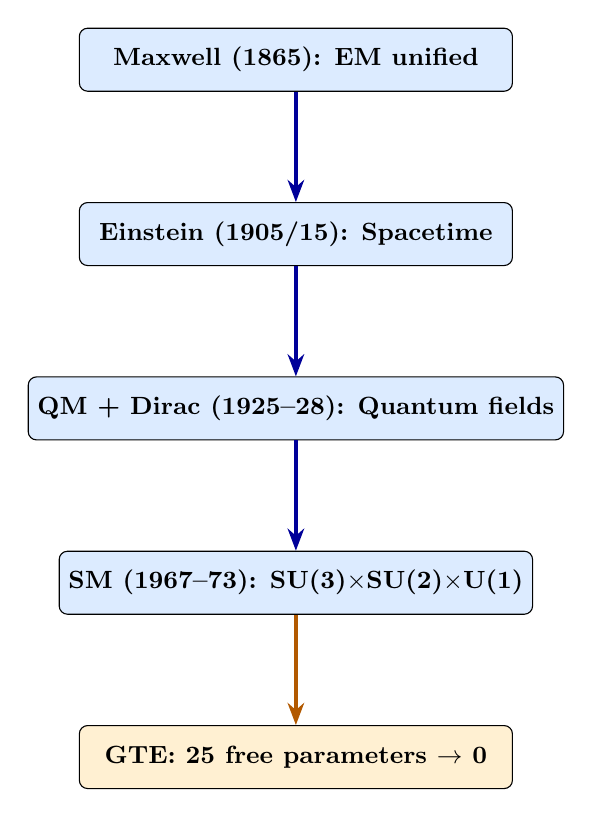
\begin{tikzpicture}[
  box/.style={draw,rounded corners=3pt,text centered,
              minimum width=5.5cm,minimum height=0.8cm,font=\small\bfseries},
  arrow/.style={-{Stealth[length=8pt,width=6pt]},line width=1.2pt,
                color=blue!60!black},
  node distance=1.4cm
]
\node[box,fill=boxblue] (maxwell) {Maxwell (1865): EM unified};
\node[box,fill=boxblue,below=of maxwell] (einstein) {Einstein (1905/15): Spacetime};
\node[box,fill=boxblue,below=of einstein] (qm) {QM + Dirac (1925--28): Quantum fields};
\node[box,fill=boxblue,below=of qm] (sm) {SM (1967--73): SU(3)$\times$SU(2)$\times$U(1)};
\node[box,fill=boxorange,below=of sm] (gte) {GTE: 25 free parameters $\to$ 0};
\draw[arrow] (maxwell)--(einstein);
\draw[arrow] (einstein)--(qm);
\draw[arrow] (qm)--(sm);
\draw[arrow,color=orange!70!black] (sm)--(gte);
\end{tikzpicture}
\caption{The historical sequence of unifications in physics.
Each step reduced the number of independent principles and produced
new predictions. The GTE framework is the next step: it converts the
SM's 25 free parameters into theorems.}
\label{fig:unification-sequence}
\end{figure}

Each historical unification reduced the free-parameter count but left a residue.
Maxwell unified electricity and magnetism, but left the speed of light
as an unexplained constant.
Einstein explained the speed of light, but left Newton's constant $G$ as an input.
Quantum mechanics explained atomic structure, but introduced the Born rule
as a postulate.
The SM unified the electroweak and strong forces, but left 25 numerical constants
without explanation.

The GTE framework closes this residue.
Table~\ref{tab:residue} shows the historical pattern.

\begin{table}[h]
\centering
\caption{Each major unification left a residue that the next step explained.
The GTE framework closes the residue of the Standard Model.}
\label{tab:residue}
\small
\begin{tabular}{lll}
\toprule
\textbf{Unification} & \textbf{What it unified} & \textbf{Residue left behind} \\
\midrule
Maxwell (1865) & Electricity + magnetism & Speed of light unexplained \\
Einstein SR (1905) & Mechanics + EM & Newton's $G$ unexplained \\
Einstein GR (1915) & Gravity + spacetime & $G_N$ as free parameter \\
QM (1925) & Atomic phenomena & Born rule postulated \\
Yang-Mills (1954) & Gauge principle & Which gauge group? \\
Electroweak (1967) & EM + weak force & $\sin^2\theta_W$ free \\
QCD (1973) & Strong force & $\alpha_s$, quark masses free \\
SM complete (1974) & SU(3)$\times$SU(2)$\times$U(1) & 25 free parameters \\
\textbf{GTE} & PSC $\to$ MDL $\to$ all SM + GR + QM & Open: $\theta_{23}$ tension \\
\bottomrule
\end{tabular}
\end{table}

%─────────────────────────────────────────────────────────────────────────────
\section{The GTE Approach: Perfect Self-Containment as the Selection Principle}
\label{sec:gte}
%─────────────────────────────────────────────────────────────────────────────

\begin{tcolorbox}[colback=boxblue,colframe=blue!40!black,
  title=The selection principle in one sentence]
The universe must be the shortest complete self-consistent description of itself.
There is exactly one such description.
It is the 19-bit polynomial $p(L,C,R) = C + R - CR - LCR \pmod{7}$.
\end{tcolorbox}

The \term{Generative Triple Evolution (GTE)} framework is built on three ideas.

\textbf{1. Perfect Self-Containment (PSC).}
The universe has no outside.
Therefore it must contain its own complete description.
This is not a metaphysical slogan but a formal axiom with mathematical
consequences~\cite{SpivackGTECompleteFramework}.

\textbf{2. Presentation Invariance (PI).}
The universe's description cannot depend on the language used to write it.
A universe described in metric units and one described in imperial units
are the same universe.
PI is a symmetry requirement on the self-description.
The theorem PI $\equiv$ MDL proves that Presentation Invariance is logically
equivalent to Minimum Description Length: the self-description must be
as short as possible.
Intuitively: if two descriptions of the same universe have different lengths,
one contains redundant information; the shorter one is presentation-invariant
and the longer one is not.
Therefore the unique presentation-invariant self-description is the shortest one.

\textbf{3. MDL selects a unique structure.}
Among all possible mathematical structures that could be the universe's
self-description, which one has the shortest description?
The answer, proved as a machine-certified theorem, is
$\mathbb{Z}_7 \times \mathbb{Z}_3$: a specific finite group
that encodes a 7-state cellular automaton rule of the form
$p(L,C,R) = C + R - CR - LCR$ (arithmetic mod 7).
The key MDL uniqueness result
(\lean{mdl\_total\_z7z3\_strictly\_beats\_z5z3}, \CatAL)
eliminates every competing structure by proving each has a longer description.

From this 19-bit structure, the GTE framework derives --- rather than fits ---
the entire SM~\cite{SpivackGTECompleteFramework,SpivackSM}.

\subsection{Why this is not numerology}

The standard objection to any program that derives particle masses from
abstract mathematics is that it is numerology: post-hoc fitting dressed up
as theory.
The GTE framework is not in that category for five reasons.

\textbf{Machine verification.}
Every foundational claim is proved in Lean~4 with zero sorry.
Lean~4 has no knowledge of the Standard Model.
It checks arithmetic on finite groups.
A machine that does not know what an electron is cannot construct a
numerological fit for the electron mass.

\textbf{Competitor elimination.}
GTE does not merely propose $\mathbb{Z}_7 \times \mathbb{Z}_3$; it proves
every alternative is worse by an explicit, machine-verified criterion.

\textbf{Zero free parameters.}
The 19-bit polynomial was not chosen because it agrees with particle physics.
Its description length $K_{\rm CA} = 19$ bits is a mathematical property
of the polynomial, independent of any physical measurement.

\textbf{Non-circularity.}
The derivation of $\mathbb{Z}_7 \times \mathbb{Z}_3$ uses no SM input.
This is enforced by the machine proof.

\textbf{Predictions before confirmations.}
Several results were derived before comparison to experiment.
The spectral tilt formula $n_s = 1 - \ln 2 / (2\pi^2) = 0.96488$ was
derived from binary holographic entropy counting and compared to
Planck~2018 at $-0.005\sigma$~\cite{SpivackGTECosmology}.

%─────────────────────────────────────────────────────────────────────────────
\section{What a Solution Would Look Like}
\label{sec:solution}
%─────────────────────────────────────────────────────────────────────────────

A complete solution to the parameter problem has four signatures.

\textbf{Zero free parameters.}
All 25 SM constants are outputs of the derivation, not inputs.

\textbf{Machine-certified derivation chain.}
Every step from the foundational axioms to the physical predictions is a
formally verified theorem.
No informal argument can slip in an assumption that implicitly imports
the known answer.

\textbf{Predictions at sub-sigma precision.}
The framework must not merely order-of-magnitude reproduce the SM constants.
It must predict them with a precision comparable to the measurement error.

\textbf{Falsifiable beyond the SM.}
A genuine solution makes predictions that go beyond reproducing known values.
It predicts things that have not yet been measured, in a way that would
definitively falsify the framework if the predictions fail.

\begin{tcolorbox}[colback=boxgreen,colframe=green!50!black,
  title={The GTE scorecard (from P48~\cite{SpivackGTECompleteFramework})},breakable]
\begin{itemize}[itemsep=2pt]
  \item \textbf{Zero free parameters:} \checkmark\ All SM constants are theorems.
  \item \textbf{Machine-certified:} \checkmark\ 308 Lean~4 modules, zero sorry,
        zero custom axioms.
  \item \textbf{Sub-sigma precision:}
        Approximately 37 of 40+ tested predictions are within $1\sigma$
        of PDG~2024 or NuFIT~6.0.
  \item \textbf{Falsifiable predictions:} \checkmark\ $r = 0$ (no primordial
        gravitational waves), $\Sigma m_\nu = 59.4$~meV, no SUSY, no axion,
        no new physics below $\Lambda_{\rm GTE} \approx 2$~GeV.
\end{itemize}
\end{tcolorbox}

The companion tutorials in this series develop each part of the derivation chain.
\emph{The GTE Polynomial: A Step-by-Step Cheat Sheet}~\cite{SpivackTutorialPolynomial} introduces the
polynomial $p(L,C,R)$ and explains why it is unique.
\emph{Perfect Self-Containment and MDL}~\cite{SpivackTutorialPSCMDL} develops the foundational principle.
The subsequent tutorials cover the particle spectrum, forces, gravity,
quantum mechanics, and cosmology.

The present tutorial has one purpose: to establish that there is a
genuine problem, and that the problem has a structure that a genuine
solution must address.
That problem is the 25 free parameters of the Standard Model.
The GTE framework proposes --- and machine-certifies --- that none of them
are free.

%─────────────────────────────────────────────────────────────────────────────
\section*{Further Reading}
%─────────────────────────────────────────────────────────────────────────────
\begin{tcolorbox}[colback=orange!8,colframe=orange!50!black,
  title=\textbf{Primary Sources}]
The results in this tutorial are derived in the following papers,
all available open-access on Zenodo and at
\href{https://novaspivack.com/research}{novaspivack.com/research}:
\begin{itemize}[itemsep=2pt]
  \item \textbf{P48 --- The Complete GTE Framework} (main synthesis monograph):\\
        \href{https://doi.org/10.5281/zenodo.20560550}{doi.org/10.5281/zenodo.20560550}
  \item \textbf{P01 --- Standard Model Parameters from the UGP} (first-principles SM derivation):\\
        \href{https://doi.org/10.5281/zenodo.20168787}{doi.org/10.5281/zenodo.20168787}
  \item \textbf{P40 --- GF(7) Polynomial Universality} (MDL uniqueness theorem):\\
        \href{https://doi.org/10.5281/zenodo.20417566}{doi.org/10.5281/zenodo.20417566}
\end{itemize}
Lean~4 machine proofs: \href{https://github.com/novaspivack/ugp-lean}{github.com/novaspivack/ugp-lean}
\end{tcolorbox}

\bibliographystyle{unsrtnat}
\bibliography{../../papers/bib/Spivack_Papers_Bibliography}

\end{document}
